%%%%%%%%%%%%%%%%%%%%%%%%%%%%%%%%%%%%%%%%%%%%%%%
\chapter{Citizen-powered Knowledge Work: Why and how?}

\begin{quote}
\emph{This dissertation explores how }
\end{quote}
\vspace{0.25in}


\section{The Challenge: People don't know how to}
\subsection{Problem Dimensions: lack of expertise, lack of time, too much work}
Harnessing humanity's collective efforts accomplishes great goals
-- start with the von Ahn example

My research raises the question: how can global communities create knowledge that meets their goals without waiting for experts to lead? My research prototypes collective systems for large-scale problems.

\section{Thesis: Procedural Support for Roles}

Many people have strong personal motivations and contextual insights. To create knowledge,
they need mental scaffolds for organizing complex work, domain knowledge to compose and
execute the steps, and ways to ask for help. Professional scientists benefit from conceptual
knowledge, professional training, pre-existing organizational structure for collaboration, and direct access to resources. Currently, citizens lack these resources.

Building on these new participation channels, we suggest that democratizing experimentation may
also expand the gamut of scientific knowledge. People have questions about their health, but lack
the expertise and resources to scientifically investigate them. How might online systems support
more complex activities that leverage the creativity and diversity of a global community?

This dissertation explores challenges people face xxxxxxx. Underlying these investigations is the thesis:

"My thesis statement is"
\begin{quote}
\emph{Understanding how the tension between exploring data and explaining process manifests itself in practice makes it possible to design software that enables analysts to document and share their work more effectively.}
\end{quote}

 \subsection{Developing an intuition}


\section{Contributions}
"This dissertation makes contributions in a number of areas. Some contributions are theoretical:
1. a model of complex tasks and dividing them to different tasks for self, community, and machines

\subsection{Theoretical: Techniques and Framework}
1. Principles to Integrate Learning in Social Computing
	1. deeper work — more learning   //     more work — better collaboration
2. Roles Support via Just-in-time Skill Acquisition
3. Framework: A different human-machine integration way 
  that puts people in the driving category, supported by algo
 Systems that divide the task between people, community, and machines

//Philosophical -- how does this research think and imagine differently; and how that was operationalized as techniques as systems
-- People have an amazing breadth and depth of ideas and work with them

All these techniques have been put in systems

\subsection{System Design (including Interfaces)}
1. UIs that integrate learning and focused collaboration
2. 

\subsection{Empirical Results from Real-world Deployment}
expertise: limited; diversity: different countries; scale: some


\subsection{Dataset}

A Venn diagram showing the contributions and the domains

This dissertation has four types of contributions: empirical results, theoretical perspectives, prototype systems, and an open dataset. Here I summarize these contributions in the order they will be presented in the chapters that follow (Figure \ref{fig:contributions}).

\begin{figure}[t!] 
  \centering
    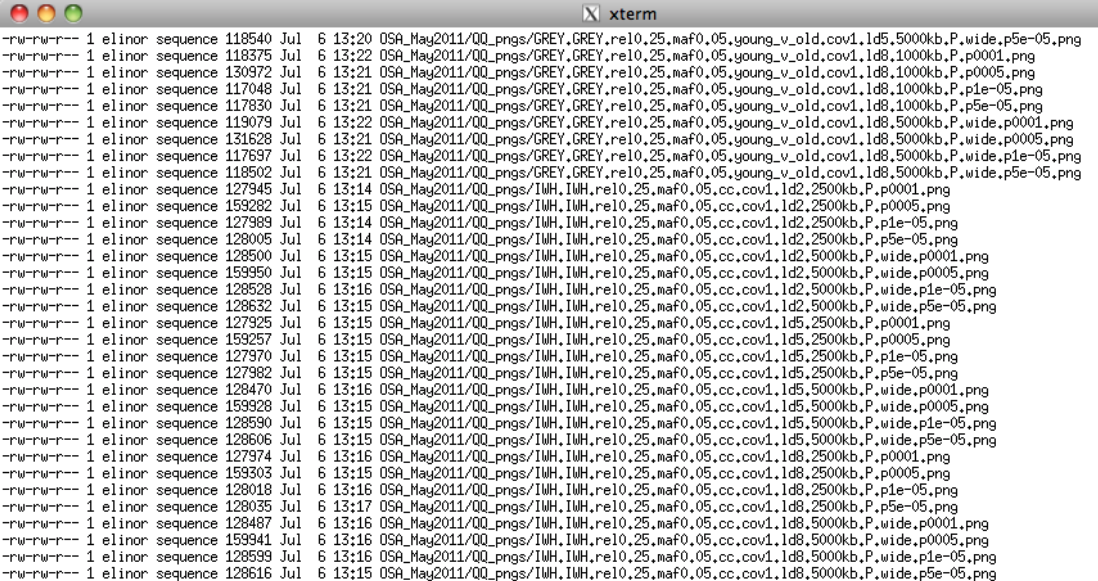
\includegraphics[width=1.0\textwidth]{img/files}
  \caption[Contributions of this dissertation]
{Contributions of this dissertation including empirical results, prototype systems, theoretical perspectives, and an open dataset.}
  \label{fig:contributions}
\end{figure}

\section{Impact}
 \subsection{Used by communities}
 \subsection{Talks in the Research community and other communities}
 \subsection{Taught in classes}


\section{Dissertation Roadmap}

%%%%%%%%%%%%%%%%%%%%%%%%%%%%%%%%%%%%%%%%%%%%%%%%%%%%%%%%%%%%%%%%%%

\chapter{Related Work}

\begin{quote}
\emph{This dissertation explores how }

\end{quote}
\vspace{0.25in}

\section{Social Computing: Elevating the Discourse}
\subsection{Systems and architectures for crowdsourcing complex work}

poor signal-to-noise from crowds due to lack of training; inefficient collaboration without careful attention; and poor results (or no results at all) unless experts lead. To address these concerns, my work introduces and evaluates peer production architectures and procedural learning

1. Meaningful social computing systems need learning
    1. my work shows how to inject learning in social computing systems


1. What is the purpose of building social computing systems?
-- probe an idea and see how far it goes (See msb)
2 .open-ended, creative tasks
3. 1. Improve the quality of poor contributions — and improve the quality of max contributions 
    1. — hockey stick curve 
4. 1. 
    1. lowers the threshold for designing an experiment - how: procedural learning
    2. support reviewing and running an experimentation with system support

\section{Online learning research focuses on conceptual understanding of class topics}
-- JIT learning techniques embedded in people’s doing

Current online learning scales the classroom but the world is not a classroom
Introduce ideas about Bloom's and Arlington -- what they should use it for
2. JIT learning techniques can be super useful
3. personally meaningful learning

\section{End-user programming has focused on technology/writing tasks}
-- A new domain for end-user programming 
End users as designers

-- Thinking differently about hci 
  people are not just information processing machines
  people are social, have motivations and goals

1. HCI work focuses on programmers, end-user programmers, "even casual users” - individuals
2. also, these tasks are CS specific (like writing)
3. we focus on a general-purpose task (like experimentation), on novices, and on communities


\section{Lead-user Innovation: Successful when People Know What to Do and How to Do It}
-- Techniques and systems to build expertise in people (toolkit?)

1. GitHub: enables storing code, sharing code, great, but doesn’t teach how to program
2. Technology systems currently use existing capacity and takes away the context that they have — how do you build capacity — people have the context 
3. techniques to build expertise in people
4. difference between lead users and end users? 
5. examples: UN example (see eric vh)

\section{The Future of Citizen Science: Running own experiments?}
-- An expansion of the depth and breadth of work performed by citizen science communities

science is nascent, highly contextual, and personally motivating.
1. Internet-scale science misses people’s lived experience \\
 “Other people’s noise is my signal” \\
2. Can people be scientists rather than just sensors? \\
 Provide a taxonomy of sorts of citizen science work
3. Scaling up science: How open is open science? \\
 open science things assume people know the science — it’s not a right assumption — providing notebooks and books does nothing // truly open science means people know how science works
4. Microbiome research: a petri dish for making scientists \\
5. link my research with more hardcore science

\section{Self-tracking Offers Insights but Not Causality}
??????

%%%%%%%%%%%%%%%%%%%%%%%%%%%%
\chapter{Collaboratively generating hypotheses}
Source of hypothses: data seen, intuitions, folk theories, experiences

\section{Learn-Train-Ask: From Intuitions to Hypotheses}
\section{Design process: CHI 2017 Gut Instinct}
People created vague unfalsifiable hypotheses

\section{Docent: System Design}
\section{Evaluation: Scaffolds For Better Questions}
 \subsection{Hypotheses Test}
 \subsection{The effect of learning and training on questions}
 \subsection{Which topics did the questions deal with?}
 \subsection{How novel are the questions?}
 \subsection{Emergent behavior, Engagement, and Growth}

\section{Discussion and Design Implications????}
\section{Summary???}



%%%%%%%%%%%%%%%%%%%%%%%%%%%%%%%%%%
\chapter{Collaboratively running experiments}

\section{Motivation}
3 reasons: people created novel hypo, people discuss on online fora, people can track fine-grained data, people are motivated to find answers


\section{Design-Review-Run: From Intuitions to Investigations}
\subsection{Techniques: Roles and Rules}

\section{Design process}

\section{Galileo system design}

\section{Evaluation}
\subsection{Study 1: Experiment Comparing Procedural Training To Videos}
\subsection{Study 2: People Design And Review Experiments Online}
\subsection{Study 3: Three Communities Design, Review, \& Run Experiments}

\section{Discussion and Design Implications????}
\section{Summary???}

%%%%%%%%%%%%%%%%%%%%%%%%%%%%%%%%%%
\chapter{Conclusion and Future Work}

\section{Theoretical Questions}

\section{New Systems?}

\section{Other areas of application?}




